\section{Thực nghiệm}
\label{sec:experiments}

% -----------------------------------------------------------------------
\subsection{Thiết lập thực nghiệm}

\textbf{Dataset.}
Thực nghiệm được tiến hành trên hai ảnh grayscale chuẩn từ thư viện scikit-image: ảnh \textit{Camera} ($512\times512$ pixel, giàu cạnh và texture) và ảnh \textit{Coins} ($303\times384$ pixel, cạnh tròn và gradient smooth). Ảnh nhiễu được tạo bằng cách cộng thêm nhiễu Gaussian với ba mức $\sigma \in \{10, 20, 30\}$, tương ứng với SNR thấp, trung bình và cao.

\textbf{Các phương pháp so sánh.}
Bảy phương pháp được đánh giá:
\begin{itemize}
    \item \textbf{DWT-Bayes:} Baseline --- wavelet thresholding với BayesShrink, wavelet db4, 3 level (scikit-image).
    \item \textbf{DFB-SURE:} DFB 8 band + LP/HP split + SURE threshold.
    \item \textbf{DFB-GCV:} DFB 8 band + LP/HP split + GCV threshold.
    \item \textbf{DFB-MAD:} DFB 8 band + LP/HP split + MAD + universal threshold.
    \item \textbf{DFB-Bayes (Cải tiến 1):} DFB 8 band + LP/HP split + BayesShrink.
    \item \textbf{DFB-Bayes-16 (Cải tiến 2):} DFB 16 band + LP/HP split + BayesShrink.
    \item \textbf{MS-DFB-Bayes (Cải tiến 3):} Multi-scale undecimated DFB, $L=3$ scale, 8 band/scale, BayesShrink.
\end{itemize}

\textbf{Metrics.}
Chất lượng denoising được đánh giá qua:
\begin{itemize}
    \item \textbf{PSNR} (Peak Signal-to-Noise Ratio): $\text{PSNR} = 10\log_{10}(255^2/\text{MSE})$, tính bằng dB.
    \item \textbf{SSIM} (Structural Similarity Index): đo lường sự tương đồng cấu trúc, trong khoảng $[0, 1]$.
\end{itemize}

Mọi thực nghiệm được thực hiện với random seed cố định (seed = 42) để đảm bảo tái lập.

% -----------------------------------------------------------------------
\subsection{Kết quả định lượng}

Bảng~\ref{tab:camera} và~\ref{tab:coins} trình bày kết quả PSNR và SSIM của tất cả phương pháp trên ảnh Camera và Coins.

\begin{table}[H]
\centering
\caption{PSNR (dB) / SSIM trên ảnh \textit{Camera} ($512\times512$). Số in đậm là tốt nhất.}
\label{tab:camera}
\setlength{\tabcolsep}{6pt}
\begin{tabular}{@{}lcccccc@{}}
\toprule
\multirow{2}{*}{\textbf{Phương pháp}}
  & \multicolumn{2}{c}{$\sigma = 10$}
  & \multicolumn{2}{c}{$\sigma = 20$}
  & \multicolumn{2}{c}{$\sigma = 30$} \\
\cmidrule(lr){2-3}\cmidrule(lr){4-5}\cmidrule(lr){6-7}
  & PSNR & SSIM & PSNR & SSIM & PSNR & SSIM \\
\midrule
Nhiễu       & 28.13 & 0.7008 & 22.11 & 0.4306 & 18.58 & 0.2939 \\
DWT-Bayes   & \textbf{31.67} & 0.8276 & \textbf{28.40} & 0.7060 & \textbf{26.86} & 0.6377 \\
DFB-SURE    & 30.09 & \textbf{0.8342} & 27.22 & \textbf{0.7424} & 26.07 & \textbf{0.6891} \\
DFB-GCV     & 28.68 & 0.6287 & 25.02 & 0.4630 & 21.06 & 0.2959 \\
DFB-MAD     & 26.78 & 0.7570 & 25.80 & 0.7191 & 25.47 & 0.6797 \\
DFB-Bayes   & 28.84 & 0.8075 & 25.70 & 0.7180 & 25.45 & 0.6796 \\
DFB-Bayes-16  & 28.97 & 0.8065 & 25.70 & 0.7180 & 25.45 & 0.6796 \\
MS-DFB-Bayes  & 27.84 & 0.7780 & 25.70 & 0.7181 & 25.45 & 0.6800 \\
\bottomrule
\end{tabular}
\end{table}

\begin{table}[H]
\centering
\caption{PSNR (dB) / SSIM trên ảnh \textit{Coins} ($303\times384$). Số in đậm là tốt nhất.}
\label{tab:coins}
\setlength{\tabcolsep}{6pt}
\begin{tabular}{@{}lcccccc@{}}
\toprule
\multirow{2}{*}{\textbf{Phương pháp}}
  & \multicolumn{2}{c}{$\sigma = 10$}
  & \multicolumn{2}{c}{$\sigma = 20$}
  & \multicolumn{2}{c}{$\sigma = 30$} \\
\cmidrule(lr){2-3}\cmidrule(lr){4-5}\cmidrule(lr){6-7}
  & PSNR & SSIM & PSNR & SSIM & PSNR & SSIM \\
\midrule
Nhiễu        & 28.13 & 0.6784 & 22.11 & 0.3839 & 18.58 & 0.2428 \\
DWT-Bayes    & \textbf{30.79} & 0.8299 & \textbf{26.88} & \textbf{0.6946} & \textbf{24.88} & \textbf{0.5999} \\
DFB-SURE     & 29.41 & \textbf{0.8402} & 25.48 & 0.7170 & 24.05 & 0.6508 \\
DFB-GCV      & 28.51 & 0.6952 & 22.71 & 0.4691 & 21.25 & 0.3881 \\
DFB-MAD      & 24.70 & 0.7025 & 23.60 & 0.6576 & 23.36 & 0.6295 \\
DFB-Bayes    & 30.17 & 0.8511 & 23.51 & 0.6553 & 23.35 & 0.6294 \\
DFB-Bayes-16 & 30.20 & 0.8481 & 23.51 & 0.6553 & 23.35 & 0.6294 \\
MS-DFB-Bayes & 27.77 & 0.7976 & 23.51 & 0.6552 & 23.35 & 0.6295 \\
\bottomrule
\end{tabular}
\end{table}

% -----------------------------------------------------------------------
\subsection{Kết quả định tính}

Hình~\ref{fig:visual_comparison} so sánh trực quan kết quả denoising của các phương pháp chính trên ảnh Camera tại $\sigma = 20$ (vùng crop trung tâm $128\times128$).

\begin{figure}[H]
    \centering
    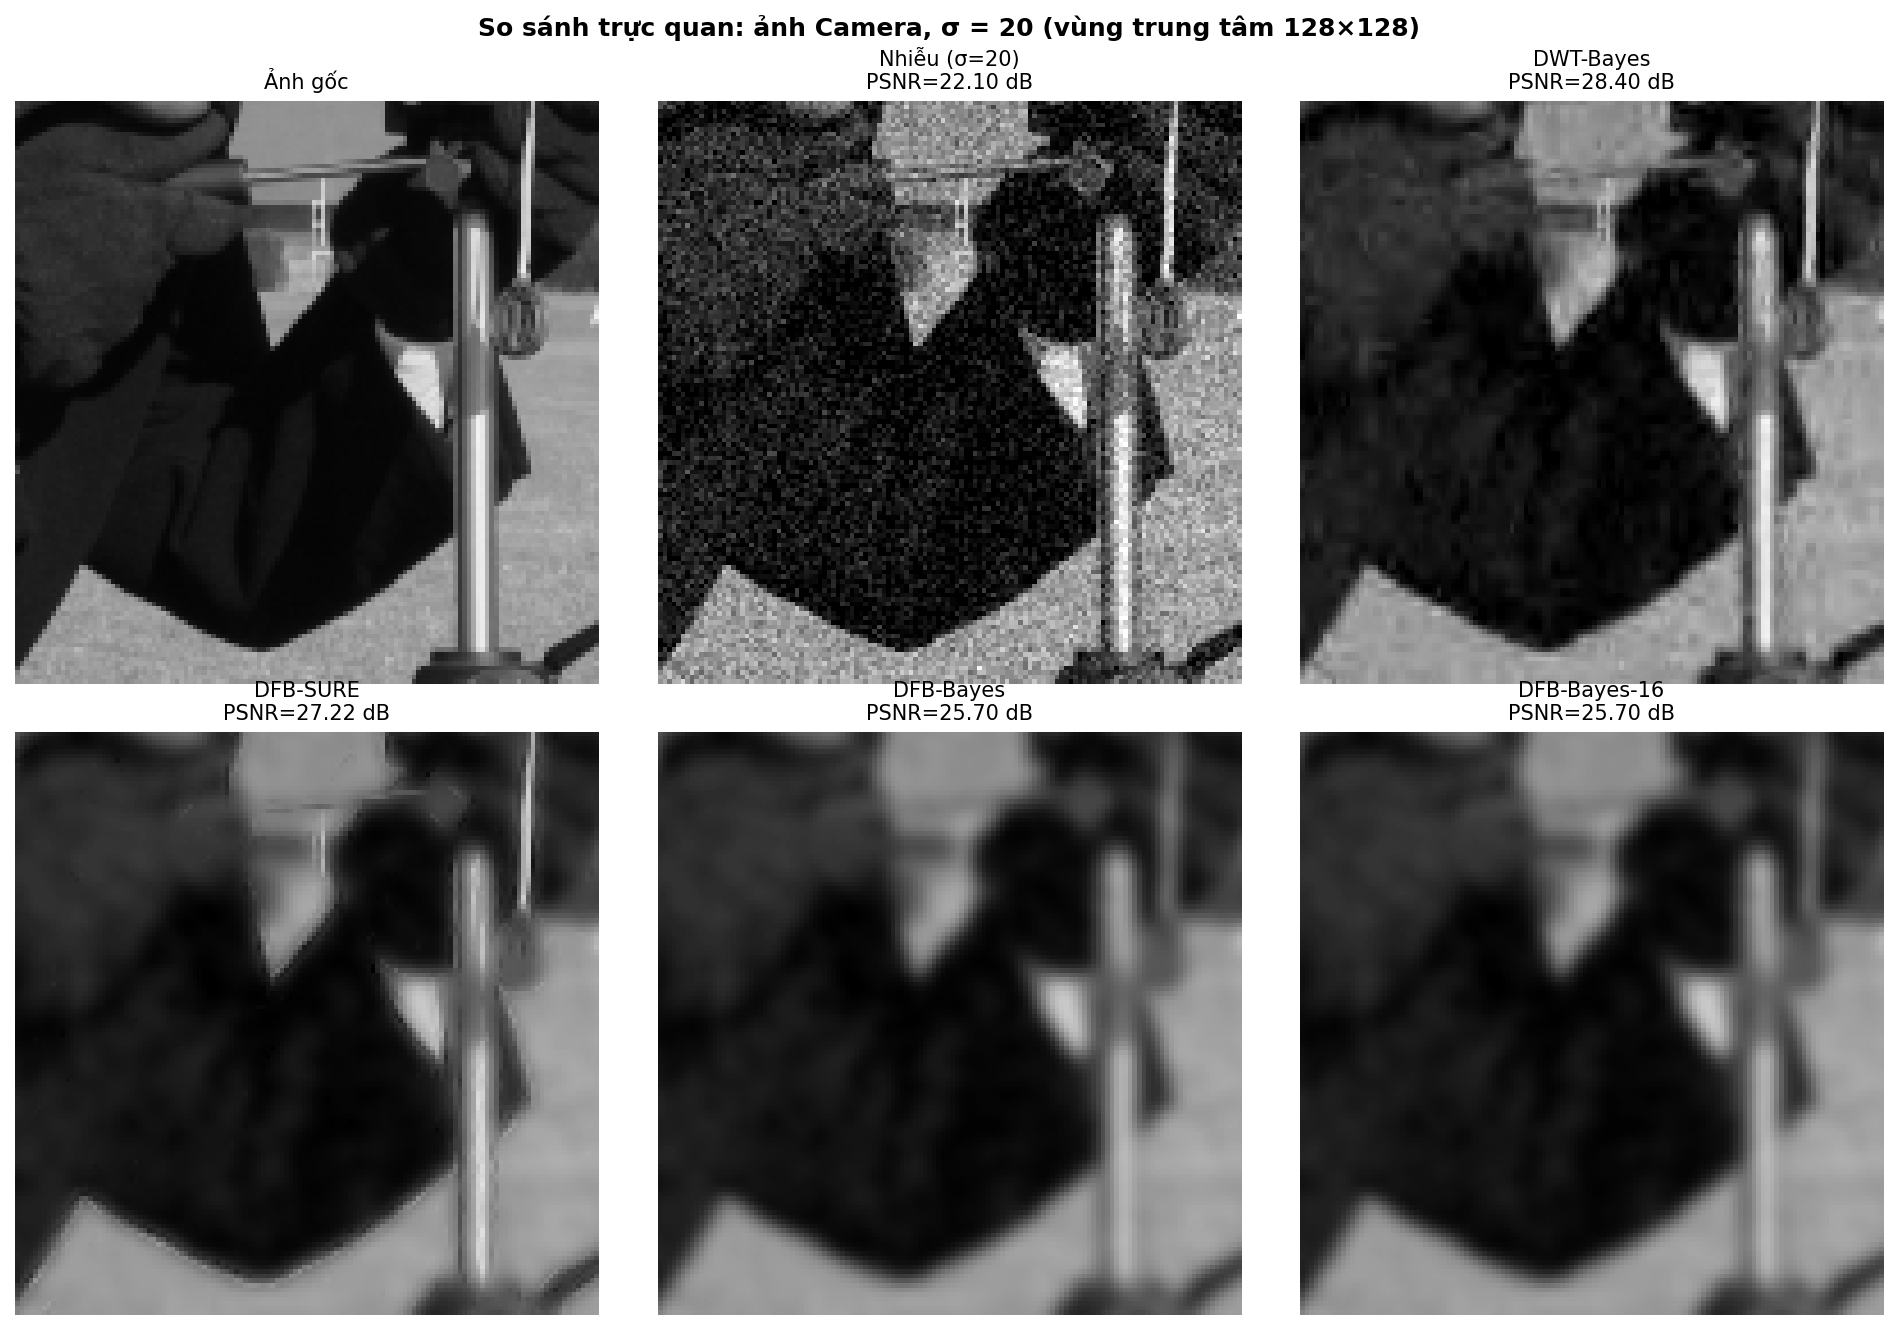
\includegraphics[width=\textwidth]{figures/visual_comparison.png}
    \caption{So sánh trực quan kết quả denoising trên ảnh Camera ($\sigma = 20$, vùng trung tâm $128\times128$).
             Hàng trên: ảnh gốc, ảnh nhiễu, DWT-Bayes.
             Hàng dưới: DFB-SURE, DFB-Bayes (8 band), DFB-Bayes-16 (16 band).}
    \label{fig:visual_comparison}
\end{figure}

% -----------------------------------------------------------------------
\subsection{Phân tích theo mức nhiễu}

Hình~\ref{fig:psnr_bars} và~\ref{fig:psnr_sigma} mô tả xu hướng PSNR theo phương pháp và mức nhiễu trên ảnh Camera.

\begin{figure}[H]
    \centering
    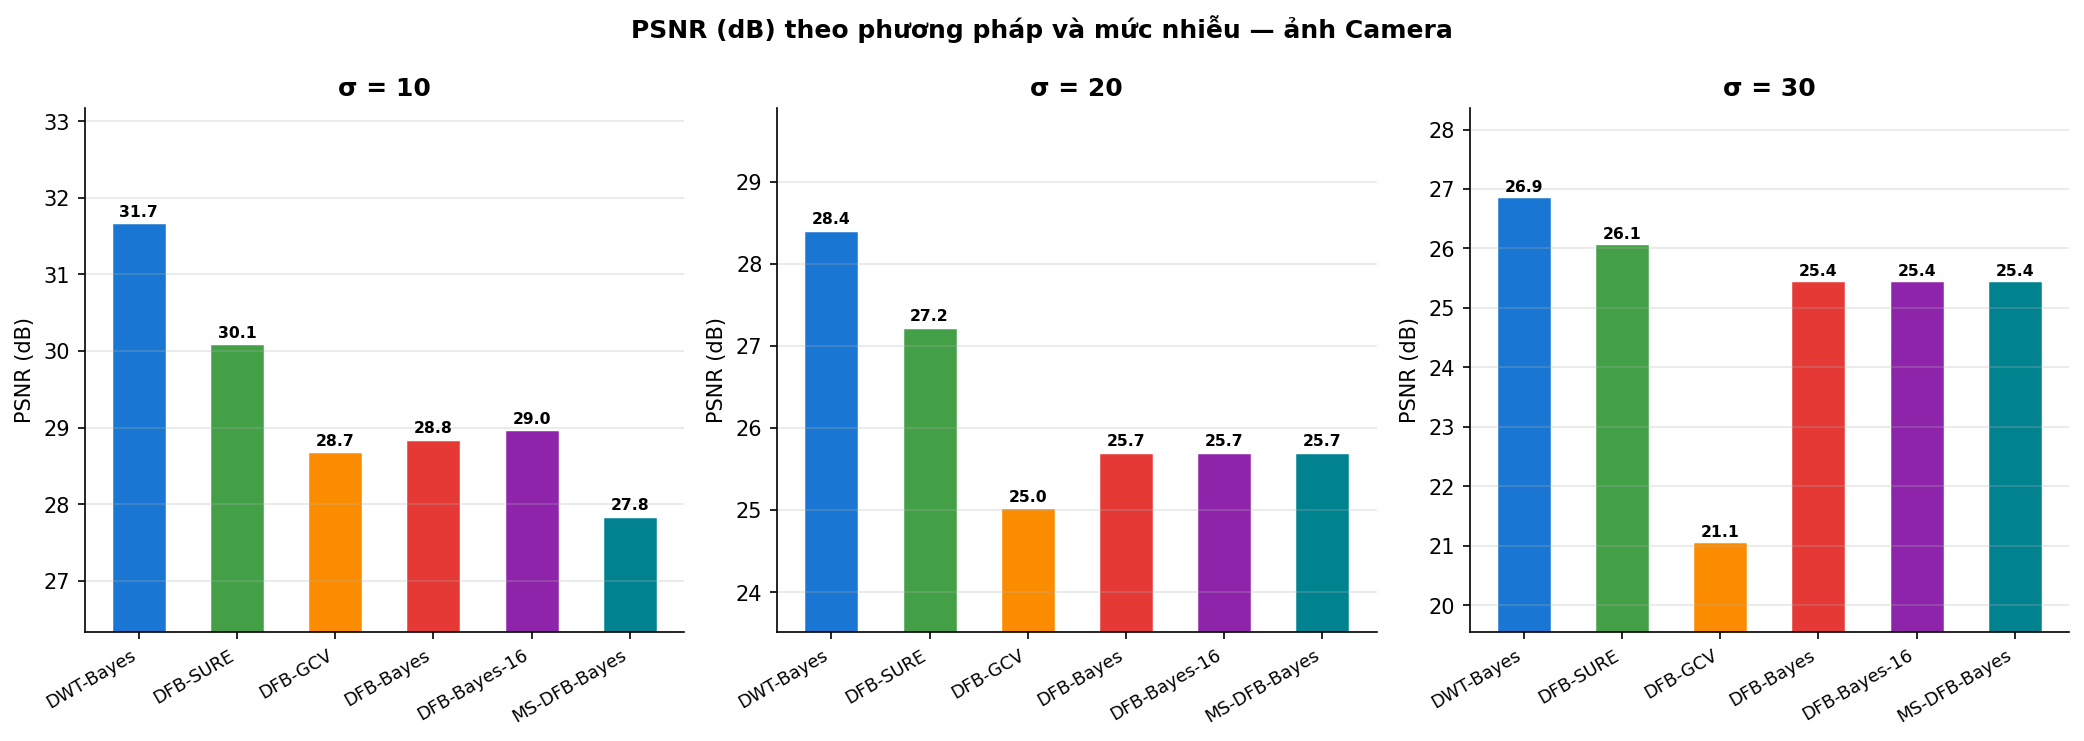
\includegraphics[width=\textwidth]{figures/psnr_comparison.png}
    \caption{PSNR (dB) của các phương pháp tại $\sigma \in \{10, 20, 30\}$ trên ảnh Camera.}
    \label{fig:psnr_bars}
\end{figure}

\begin{figure}[H]
    \centering
    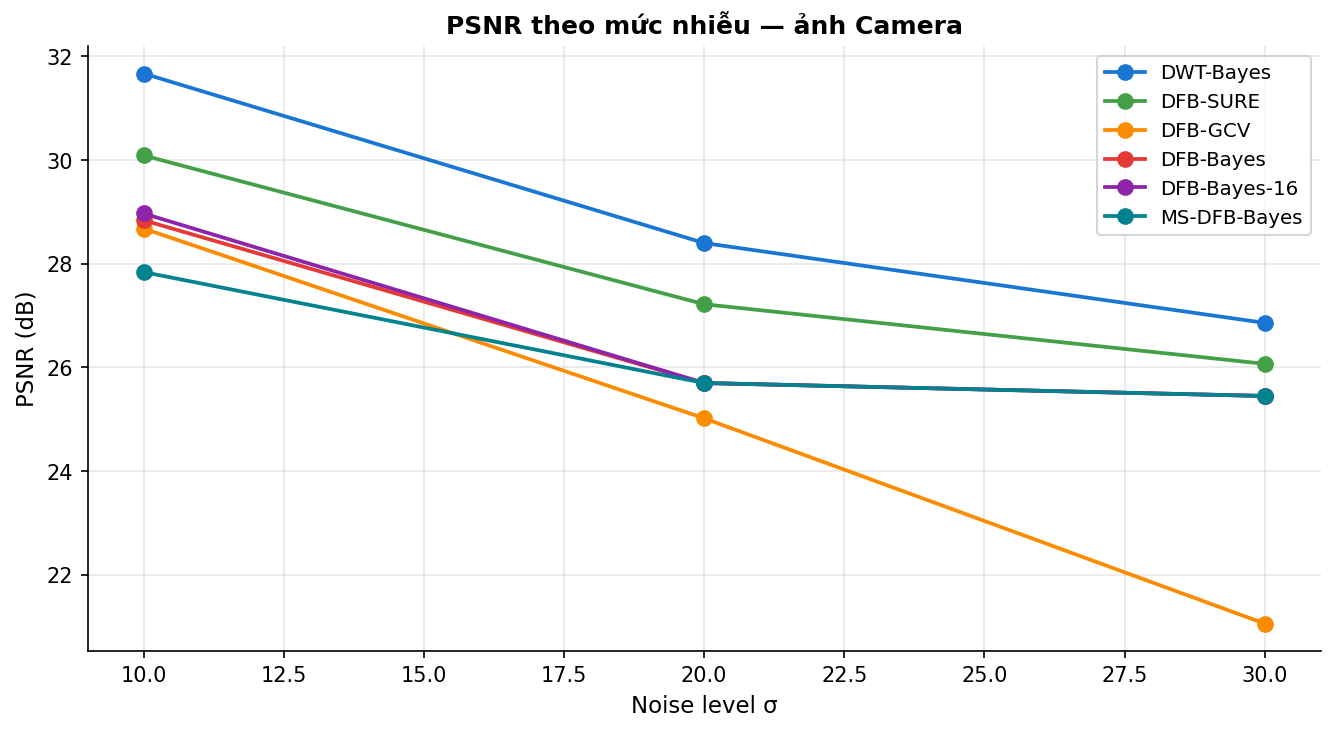
\includegraphics[width=0.75\textwidth]{figures/psnr_vs_sigma.png}
    \caption{PSNR theo mức nhiễu $\sigma$ của các phương pháp trên ảnh Camera.}
    \label{fig:psnr_sigma}
\end{figure}
